\documentclass[journal]{IEEEtran}
\usepackage{amsmath,amssymb,amsfonts}
\usepackage{tabularx}
\usepackage[utf8]{inputenc} % allow utf-8 input
\usepackage[T1]{fontenc}    % use 8-bit T1 fonts
\usepackage{url}            % simple URL typesetting
\usepackage{booktabs}       % professional-quality tables
\usepackage{amsfonts}       % blackboard math symbols
\usepackage{nicefrac}       % compact symbols for 1/2, etc.
\usepackage{microtype}      % microtypography
\usepackage{graphicx}
\usepackage{float}
\restylefloat{table}
\usepackage{hyperref}
\usepackage{multicol}
\usepackage{caption}
\usepackage{subcaption}
\usepackage{amsmath}
\usepackage{algorithm}
\usepackage{algpseudocode}
\usepackage{tikz}
\usetikzlibrary{trees}
\usepackage{listings}

\DeclareMathOperator*{\argmax}{arg\,max}  % in your preamble
\DeclareMathOperator*{\argmin}{arg\,min}  % in your preamble

\usepackage{textcomp}


%\usepackage[retainorgcmds]{IEEEtrantools}
%\usepackage{bibentry}
\usepackage{xcolor,soul,framed} %,caption

\usepackage[noadjust]{cite}
%\usepackage{biblatex}
%\bibliographystyle{plain}

\usepackage[font=small]{caption}

%=== TITLE & AUTHORS ====================================================================
\begin{document}
\bstctlcite{IEEEexample:BSTcontrol}
    \title{test}
\title{A Guide to Riding the Waves of Reinforcement Learning for Control Researchers}
\author{ Zongqiang Pang,Liping Bai ~\IEEEmembership{Member,~IEEE,} \thanks{Nanjing Unversity of Posts and Telecommunications, College of Automation \& College of Artificial Intelligence, Nanjing, Jiangsu,210000 China email:zqpang@njupt.edu.cn}}
% ====================================================================
\maketitle
% === ABSTRACT ====================================================================
% =================================================================================
\begin{abstract}
This paper is aimed at providing researchers in the field of control and optimization a bridge for incorporating deep reinforcement learning into their work. Considerable amount of progress has been made in deep learning and its associated compuatational infrastructure, which makes fast and accurate approximation a possiblity. Beyond the obvious increased capacity of perception such as facial recognition and natural language processing that can be integrated into control tasks, deep reinforcement learning and the compuational capacities comes with it should be better utilized by control researchers to formulate their problems. Off the shelf implementations of various reinforcement learning agents written in either PyTorch or Tensorflow can be easily found. Yet, when control researchers venture into this subject, they would find out that there is still quite a lot caveats and pitfalls when it comes to applying neural network to optimization problems. They can't just formulate their optimization problem into reinforcement learning format and let those off the shelf agents have a go at it. We summarized how optimization problems differ from problems such as facial recognition and how the mathematical tools we use differ vary as a result. We also provide a summary of existing researches at the croassroad between optimization and reinforcement learning.
\end{abstract}
% === KEYWORDS ====================================================================
% =================================================================================
\begin{IEEEkeywords}
Reinforcement Learning, Control Theory, Optimal Control, Optimization
\end{IEEEkeywords}
% For peer review papers, you can put extra information on the cover
% page as needed:
 %\ifCLASSOPTIONpeerreview
 %\begin{center} \bfseries EDICS Category: 3-BBND \end{center}
% \fi
%
% For peerreview papers, this IEEEtran command inserts a page break and
% creates the second title. It will be ignored for other modes.
\IEEEpeerreviewmaketitle


% === I. Paper =============================================================
% =================================================================================
\section{Introduction}
\IEEEPARstart{R}{einforcement} learning is process of methotically extracting information from observations to gradually bound the policy distribution, either directly through policy gradient methods or via scafolding measurements, such that the expected reward along a trajectory is maximized. This objective is quite similar to that of Trajectory Optimization which utilizes myriade of computational techniques to incorporating scripted constraints, which capture the dynamics of a system with exquisit equations. They are the "Black Box" approach and "White Box" approach to the problem of control, neither is perfect.

The "Black Box" approach requires copious amount of data. Efforts has been made to make it more broadly applicable and more efficient. For instance, Sergey Levine utilizes unsupervised learning to build an agent with intuitions of the physical world \cite{Finn2016UnsupervisedLF}; Chelsea Finn introduced Meta-Learning \cite{Finn2017ModelAgnosticMF} to extract overaching structures embedded in similar tasks of different setting. This line of research is mostly done in the Computer Science department, and the most important tool kit for them is statistical learning theory. Despite effort from the best mathematical minds, some complicated dynamics still elude the "White Box" approach.

It is obvious that biological systems approaches control from both angles. Unfortunately, these two subjects are studied by two communities of researchers who use different notations to discribe the same processes and they publish their research only in journals of their own disciplines. In this paper, we hope to provide a bridge for researchers in the field of control theories who would like to incorporate reinforcement learning into their works.

We are not the first ones to take up this challenge. Recently, there are interdiscipline conferences held specifially for the purpose of briding the gaps between these groups of people, for instance the \href{https://l4dc.mit.edu/}{L4DC (Learning for Dynamic Control) conference} and \href{https://www.ipam.ucla.edu/programs/workshops/intersections-between-control-learning-and-optimization/}{Intersections between Control, Learning and Optimization Workshop}.

In this paper, we build on the work of Benjamin Recht \cite{Recht2018ATO} to formulate reinforcelent learning in the language of optimization. The first barrier facing control researchers is consolidating the notation between control and reinforcement learning communities. Control communities use the notation system introduced by Lev Pontryagin. State is denoted $ \mathcal{X}$, Action is denoted $\mathcal{U}$, which is the first letter of Russian for "Action", the dynamics and stocasticity is captured by physical model constraints $x_{t+1}=f(x_t,u_t,e_t)$ where e denote the noise of a system. The objective is usually to minimize the cost funtion $\mathcal{J(.)}$. Reinforcement Learning communities use the notation system introduced by Richard Bellman who studied dynamic programming. State is denoted $\mathcal{S}$, Action is denoted $\mathcal{A}$. The dynamics and stochaticity is captured via transition matrix $\mathcal{P}$ of a Markov Decision Process.The objective of RL is the maximize the reward function $\mathcal{R(.)}$. Yet, if we set the transition matrix to be identical to the noise, then it is clear that the underlying process behind these two notation system are exactly the same. The differences are nothing but style. Since the audience of our paper is the control community, we would cast reinforcement learning in the control notation system.

We would first introduce where to bring approximation into optimization and the mathematical tools we need to better formulate such approximations. We then elaborate on the enumerated path in section II and list all the papers in this area of research. There are low handing fruit for incorporating the subjects of control and reinforcement learning such as bringing vision into control, we exclude it from our paper and focusing only on bringing the approximation and computation into control.
% === II. Harmonically-Terminated Power Rectifier Analysis ========================
% =================================================================================
\section{Where to Approximate}
The constraints imposed in the Trajectory Optimization formulation manifest themselves directly in policy $\pi(x)$ and resulting in either a narrow band of trajectories or a single optimal solution. However, adjustments in the reinforecement learning formuation is not the policy per se but its distribution. Eventually, what we hope to acheive via learning is a policy distribution, either through policy gradient method or cost to go method, which would maximize the expected reward of a trajectory.

Reinforcement Learning is not a new subject, control researchers probably know it by the name Approximate Dynamic Programming. Yet the major progress in recent years is the enhanced compuation power which brought about the potential of neuronetworks as a universal approximator \cite{Hornik1991ApproximationCO} to fruition. Most notably the series of wins reinforcement agents such as AlphaGo, AlphaStar forged against the best human players in the respective disciplines.

Broadly speaking, there are three revenues where neuronetwork based approximation can find its way into optimization as shown in \ref{fig:1}. One is learning a dynamics model from samle; Second is policy gradient based learning; Third is approximation of cost to go functions such as value funtion and Q function. The details of the implementation would be specified in the subsequent sections.

\begin{figure}[H]
    \centering
    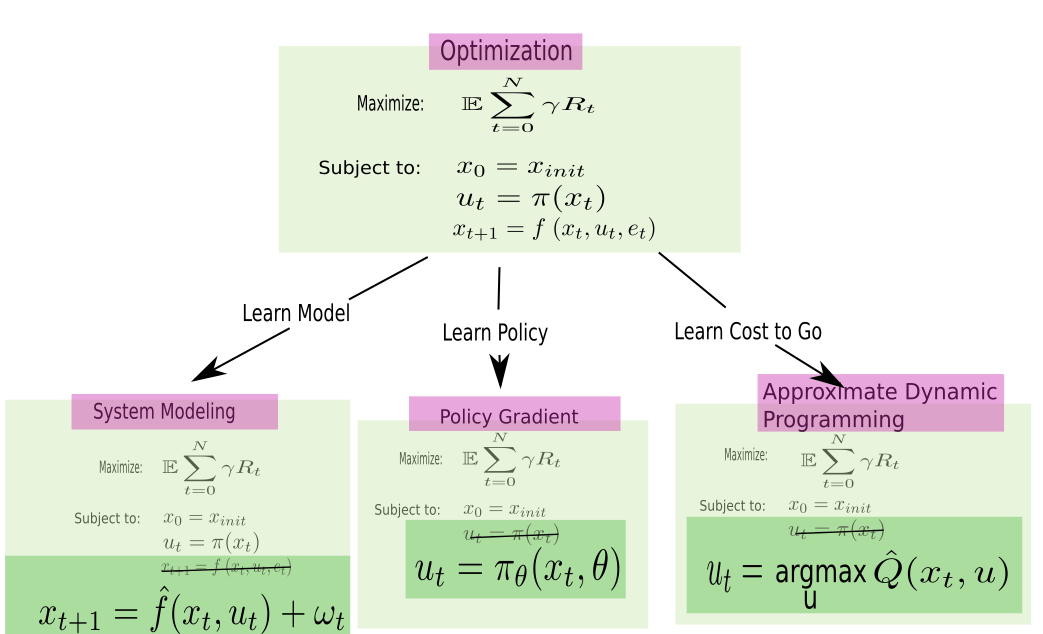
\includegraphics[width=0.5\textwidth]{Control.png}
    \caption{From Optimization to Learning}
    \label{fig:1}
\end{figure}

\section{Additional Mathematical Tools}
Before we dive into the detailed researches in each category, we'd like to introduce additional mathematical tools and measurements that has been proven useful in merging reinforcement learning with optimization. As we discussed in the previous section, the major breakthrough in the field of reinforcement learning is not necessarily the theory but the computational infrustruction. Today, reinforcement learning agents implemented with Tensorflow or PyTorch is widely available, yet if you simply formulate an optimization problem into reinforcement learning format and apply those off the shelf reinforcement learning agents, it would hardly work.

Neuronetwork based approximation in the context of optimization and control is fundamentally different from those we find in applications such as facial recognition or natual language processing. Additional mathematical tools and measurements are required to fit the structures required by control problems. While the topic of statistical learning theory is vast and profund, we selected two concepts that is most germane for bridging reinforcement learning to control theoriest. The exact use of these concept would be specified in the subsequent sections when we discuss the related papers.

\subsection{Mutual Information}
The go to text book for reinforcement learning community is that of Richard Sutton \cite{Sutton1998IntroductionTR}. In ths system contstructed by Richard, the objective of an agent is to maximize discounted reward. This formulation is proven a sound goal in the context of video games. However, for optimizations with a physics underpining, reward maximization is not adequate since noise and disturbances is common place in control.

The mathematical measurement used for mutual information \cite{Kullback1951ONIA}, which is the KL divergence. As people exposed to the measurement theory, one obvious question is that why divergence instead of distance?

\subsection{Bayesian Neuro Network (BNN)}

The venena formulation of neuronetwork is one where the weight of each neuron $w_i$ is a single number, which is adjusted based on the backward propogation process. Baysian Neuro Network is a network where the weigh is subject to a parameterized distribution as shown in Fig. \ref{fig:2} The use of Bayesian Neuro Network is to measure the uncertainly of the current iteration.
\begin{figure}[H]
    \centering
    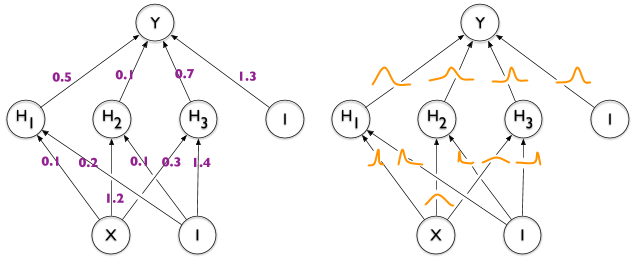
\includegraphics[width=0.5\textwidth]{bnn.png}
    \caption{Neuronet and BNN}
    \label{fig:2}
\end{figure}

\section{System Modelling}
\begin{figure}[H]
    \centering
    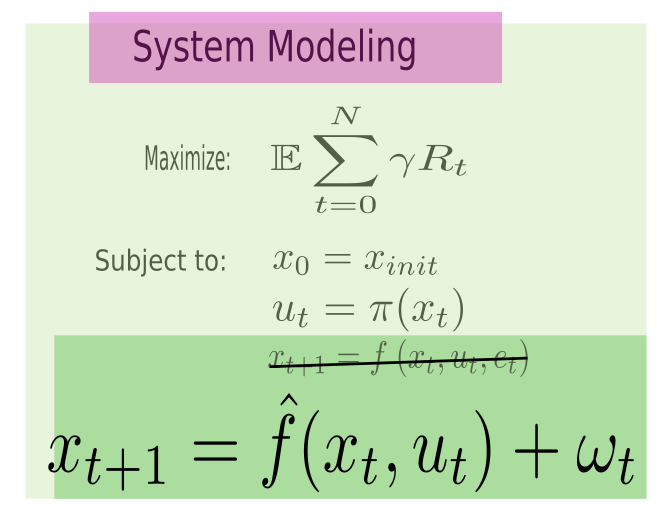
\includegraphics[width=0.3\textwidth]{Control1.png}
\end{figure}

For people who are trained in classical control theory, system modelling and system identification are the bread and butter of their field of study. One of the most obvious way to derive a model from learning is through the following althrithm:

\begin{algorithm}
\caption{Brute Force Modelling}
\begin{algorithmic}[1]

    \State run random policy, collect $\mathcal{D}=(x,u,x')_i$
    \While{Model Has Not Converged}
    \State fit model to minimize $\displaystyle \sum_i \left\|\hat{f}(x_i,u_i)-x'\right\|$
    \State Model Predictive Control using $\hat{f}(x_i,u_i)$
    \State exercute control collect new data
    \State append new data to $\mathcal{D}$
    \EndWhile

\end{algorithmic}
\end{algorithm}

\subsection{Measure Model Uncertainty with BNN}

While in theory the aforementioned brute force modelling method should work, in practice it is proven to be far from satisfactory. \cite{8463189}. One possible explanation is that any overfitting of the model would be hard to overcome, resulting in suboptimal performance. One solution is to measure uncertainly of the model with BNN.

asdfjajdflajsdlfjajdsfl;adfjlakjdflajsdflajkdfsjaldfja


\subsection{Embeded Optimization Layer and Residual Dynamics}
Writing governing equations of a physical system is something classical control theoriest trained on, yet there are always dynamics which are too intricate to be captured in full. One mental tool to deal with the uncaptured dynamics is to pack them all into a parameterized distribution which can be approximated with neuronetwork. There are two approaches in merging physics model with neuronetwork. One is to embed the optimization solver as a layer in the neuronet \cite{BelbutePeres2018EndtoEndDP} \cite{BelbutePeres2020CombiningDP} \cite{Agrawal2019DifferentiableCO}, two is to only approximate residual dynamics that can't be fully captured by the existing model \cite{Shi2019NeuralLS}.






\subsection{Safe Region}


\section{Policy Gradient}
\subsection{Trust Region Policy Iteration}
\subsection{Direct Policy Fitting}

\section{Approximate Dynamic Programming}









\subsection{Value Iteration and Policy Iteration}
\subsection{Maximum Entropy Reinforcement Learning}
Exploration and Exploitation trade off is something studied exhaustively in the reinforcement learning community. A common strategy is $\epsilon$ greedy policy where the value of epsilon decays as the learning progresses. Yet, the decaying rate is a hyperparater that need to be tuned. Is there are more sysmtmatical way to balance the exploration and exploitation trade-off? This is particularly important for control related training since this application has considerable amount of disturbance and noise. If the policy converges too soon, any subsequent disturce can deviate the trajectory to the extend that it is no longer controllable.

The intuition behind maximum entropy reinforcenement learning is the heuristic that when we don't know all the circumstance, we should prioritize options that could give us more choices regardless of how the system dynamics turns out to be. Statitically speaking, this means we should maximize the entropy of a distribution, which measures how uncertain or how broad the distributionb is.


kjhjhjhjhjh






\section{Other Ways to Utilize Increased Computational Power}
\subsection{Multiagent Formulation}
\subsection{Monte Carlo Tree Search}



\subsection{Random Shoot}
One of the corrilary of the development of reinforcement leraning is improvement in computational infrastructure, which is something the control community can take advantage of. Before this wave of hype in machine learning, GPU enabled computation was a specialty knowledge that is only accessable to large corporations. But now, with CUDA and related software, such compuational power is as easy

Random shoot is the idea if rolling out trajectory at random and wht the fuck is random shoot?












random text

\begin{figure}[H]
    \centering
    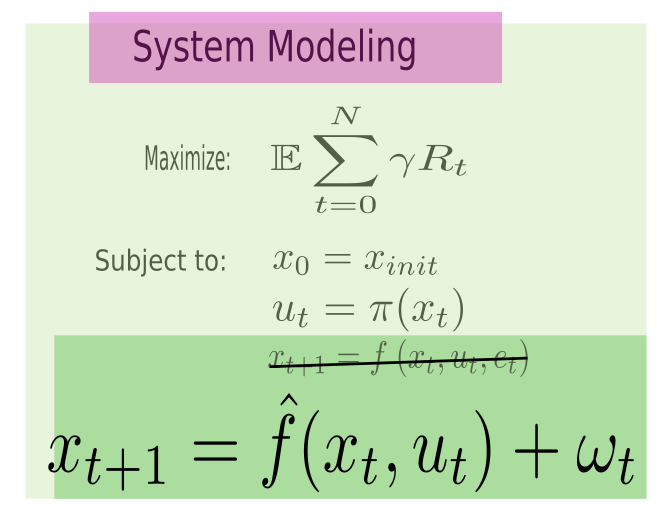
\includegraphics[width=0.2\textwidth]{Control1.png}
    \caption{Optimization}
    \label{fig:CO}
\end{figure}

\begin{figure}[H]
    \centering
    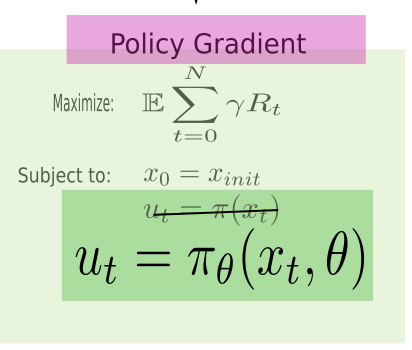
\includegraphics[width=0.2\textwidth]{Control2.png}
    \caption{System Identification}
    \label{fig:SI}
\end{figure}

\begin{figure}[H]
    \centering
    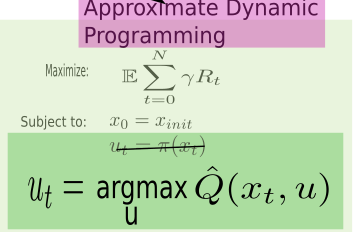
\includegraphics[width=0.2\textwidth]{Control3.png}
    \caption{Policy Gradient}
    \label{fig:PC}
\end{figure}

\begin{figure}[H]
    \centering
    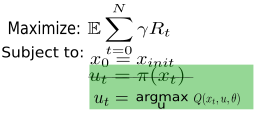
\includegraphics[width=0.2\textwidth]{Control4.png}
    \caption{Approximate Dynamic Programming}
    \label{fig:ADP}
\end{figure}



\subsection{Wireless Power Transfer}

The objective of energy beamforming control is to choose a beamforming code for each energy transmitting node such that the total received power is maximized while satisfying the minimum energy requirement of each energy receiver.

\begin{equation*}
    \begin{aligned}
        & \underset{ \textbf{f}_p, \forall p}{\text{maximize}}
        && \displaystyle\sum_{j \in \{1,2,...,L\}} e_j\\
        & \text{subject to}
        && \textbf{f}_p \in \mathcal{F}, \forall p;\\
        &&& e_j \geq e_{min}\\
    \end{aligned}
\end{equation*}


\section{Reinforcement Learning}


\subsection{problem setup}
Twritten in its recursive form, known as Bellman Equation, which is the basis for an iteratively implemented backward induction algorithm:

\begin{equation}
        G_{t}=R_{t}+\gamma G_{t+1}
    \label{bellman}
\end{equation}
Transition matrix is intruduced to encode the stochastidy in the environmental dynamics. Transaction Matrix $\mathcal{P}$ is defined as:

\begin{equation}
    \mathcal{P}_{ss'}^a := Pr\{S_{t+1}=s'|S_{t}=s,A_{t}=a\}
\end{equation}


State/Action Function q(s,a) is definied as expected gain starting from state s by taking action a:

\begin{align}
\begin{split}
    q(s,a) :&= \mathbb{E}\{G_t|S_t=s,A_t=a\}\\
    &=\mathbb{E} \{\sum_{k=0}^{T-t} \gamma ^k R_{t+k+1}| S_t=s,A_t=a\}\\
\end{split}
\end{align}
Policy is defined as:
\begin{equation}
    \pi(s,a):=Pr(A=a|S=s)
\end{equation}
Optimal Policy is defined as:
\begin{equation}
    \pi^*(s):=\argmax_a q(s,a)
\end{equation}


Value Function v(s) is defined as the expected gain starting from state s:

\begin{align}
\begin{split}
    v(s) :&=  \mathbb{E}\{G_t|S_t=s\}\\
    &=\mathbb{E} \{\sum_{k=0}^{T-t} \gamma ^k R_{t+k+1}| S_t=s\}\\
    &=\sum_{a \in \mathcal{A}} \pi(s,a) q(s,a)\\
\end{split}
\end{align}

\subsection{Without Approximation}
One obvious approach to learning is to statistically construct a model of the environment, which is called Model-Based Learning. The most primitive form of model-based learning is Bellman Equation based backward induction. Statistical tactics, such as maximum likelihood, Bayesian methods, etc., can be deployed to approximate the model with the least amount of sampling. However, since the environment is implicitly embedded in v(s) and q(s,a), the model building process can be circumvented entirely, hence Model-Free Learning. Depending on whether the iteration rules is policy dependent, model-free learning can be subdivided into on-policy learning and off-policy learning.

One hindrance to the implementation of the brute force backward induction is its memory requirement. A more effective approach is to update q value and v value after one episode, one step, or n steps. They are called Monte Carlo Method, Temporal Difference Method, and $\lambda(n)$ Method respectively.

For online learning, $\epsilon$-greedy Policy $\pi_{\epsilon}(s)$ is frequently deployed to balance exploration and exploitation, such that the environment can be encoded most efficiently. $\epsilon$ is initiated set to 1 and then asymptotically goes to 0 as the episode counts increases.

\begin{equation*}
    \pi_{\epsilon}(s,a) = \begin{cases}
        1-\epsilon+\frac{\epsilon}{|A|}& \displaystyle\argmax_{a} q_{\epsilon}(s,a)\\
        \frac{\epsilon}{|A|}& \text{otherwise}\\
           \end{cases}
\end{equation*}

\subsection{With Approximation}
When the problem gets complex, state S becomes a rather large vector and function approximation with neuro networks can be utilized to facilitate learning. Reinforcement learning as a self-sustaining mathematical framework has been refined by Rich Sutton et al. since the 1980s. Only recently, the progress made with Deep Learning has been applied to the realm of Reinforcement Learning

Let the value function and state/action function be parameterized with $\textbf{w}:  \hat{v}(s,\textbf{w}) \approx v(s)$ and $\hat{q}(s,a,\textbf{w}) \approx q(s,a) $

Let the $i^{th}$ iteration of parameter be denoted as $\textbf{$w_i$}$. The Loss Function $\mathcal{L}(\textbf{$w_i$})$ is defined as the following:
\begin{equation}
    \mathcal{L}(\textbf{$w_i$}) := \mathbb{E}\{[v(s)-\hat{v}(s,\textbf{$w_i$})]^2\}
    \label{v_loss}
\end{equation}

\begin{equation}
    \mathcal{L}(\textbf{$w_i$}) := \mathbb{E}\{[q(s,a)-\hat{q}(s,a,\textbf{$w_i$})]^2\}
    \label{q_loss}
\end{equation}
While the real value of v(s) and q(s,a) are not knowable, it can be approximated:
\begin{equation}
    v(s) \approx \sum_{a \in A} R(s,a)+\gamma v(s',\textbf{w})
    \label{v_approx}
\end{equation}
\begin{equation}
    q(s,a) \approx r+\gamma \argmax_{a} q(s',a',\textbf{w})
    \label{q_approx}
\end{equation}

The Gradient of weighing paramter \textbf{w} can be derived from \ref{v_loss} and \ref{q_loss} with the real values substituted by \ref{v_approx} and \ref{q_approx} respectively. By convention, constant is omitted. Parameter is updated following Gradient Descent:
\begin{equation}
\textbf{w}_{i}=\textbf{w}_{i-1}-\nabla_{w_{i-1}} \mathcal{L}(w_{i-1})
\end{equation}
\subsection{Policy Gradient Methods}
Policy $\pi(s)$ can be written as a function parameterized by $\theta$ with s as input and a smooth distribution overall all actions as output.By adjusting parameter $\theta$ we can adjust the distribution over action choices for different states. This style of learning is called policy gradient-based learning.

Let us register a path sequence taken by the agent as $\tau$ such that the sequence is denoted as \{$S_{\tau 0},A_{\tau 0}, R_{\tau 0}...S_{\tau T},A_{\tau T},R_{\tau T}$\}. the gain of sequence $\tau$ is defined as the gain of this entire sequence of state, action, reward:
\begin{equation}
    G(\tau):=\displaystyle\sum_{t=0}^{T}\gamma^t R_t
\end{equation}

Denote $P(\tau,\theta)$ as the probability that path $\tau$ is travesed when the policy is parameterized by $\theta$. The Objective Function can be defined in various ways. Here we adopt the definition as the following:
\begin{equation}
    U(\theta)=\sum_{\tau}P(\tau,\theta)G(\tau)
\end{equation}


The objective of the policy gradient method is to find the parameter $\theta$ to maximize the objective function.

The gradient of aforementioned utility function is:
\begin{equation}
    \nabla_{\theta} U(\theta)= \nabla_{\theta}\sum_{\tau}P(\tau,\theta) G(\tau)
\end{equation}

A mathematical sleight of hand called Importance Sampling is deployed to convert this theoretical expression of gradient into something that is algorithmically feasible.

\begin{align}
\begin{split}
\nabla_{\theta} U(\theta) \approx \frac{1}{N}\displaystyle\sum_{\tau=1}^{N}\displaystyle\sum_{t=0}^{T-1} \nabla_{\theta}ln\pi_{\theta}(s,a)|_{\theta_{old}}[q^{\pi_{\theta_{old}}}(s,a)-b]\\
\end{split}
\end{align}

We can use stochastic gradient descent(SGD) method to update $\theta$:
\begin{equation}
    \theta=\theta_{old}-\alpha \nabla_{\theta}ln\pi_{\theta}(s,a)|_{\theta_{old}}[q^{\pi_{\theta_{old}}}(s,a)-b]
\end{equation}

Actor-Critic Method takes advantage of both policy gradient and function approximation to build a bootstrap structure that lead up to fast convergence. state/action function for policy $\pi_{\theta}(s)$ is approximated by $q^{\pi_{\theta}}(s,a,\textbf{w})$.Baseline b is introduced into the bootstrap stracture to foster convergence. Different algorithms define baseline differently. In advantage Actor-Critic algorithm, baseline is defined as a value function based on $\pi_{\theta}$.Because the SGD updating process does not rely on the ordering of things, it is obvious that some of the aforementioned computations can be done asynchronously. Asynchronous Advantage Actor-Critic (A3C) is proven one of the most effective agents for renforcement learning, and is the one we will use in this paper.

\subsection{Multiagent Reinforcement Learning}
$A_t=\{A_t^1,A_t^2,...,A_t^M\}$ M is the number of agents. The action space is cartician product of action choices available to each agent. $A_t(s)=A_t^1(s) \times A_t^2(s) \times ... \times A_t^M(s)$, which grows exponentially as the number of agents grows.


Without intermidiate state rollout, the sequences of data collected is:
...$S_t, A_t, R_t, S_{t+1}$... as shown in Figure \ref{fig:without}

\begin{figure}[H]
\centering
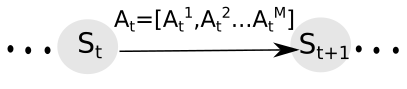
\includegraphics[width=0.3\textwidth]{without.png}
\caption{Without Rollout}
\label{fig:without}
\end{figure}

The intermediate states rollout technique converting action space complexity into state-space complexity by introducing intermediate states, denoted as $S_t^k$ where k goes from 1 to M-1. The sequence of data is now: ...$S_t,A_t^1,R_t^1,S_t^1,A_t^2,R_t^2, S_t^2, ... , S_t^{M-1},A_t^M,R_t^M,S_{t+1}$... as shown in Figure \ref{fig:with}

\begin{figure}[H]
\centering
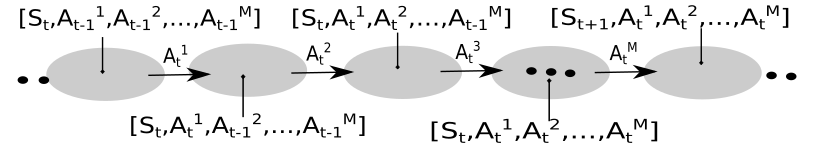
\includegraphics[width=0.55\textwidth]{with.png}
\caption{With Rollout}
\label{fig:with}
\end{figure}
suppose each agent has N choices. This formulation reduces the size action space from $N^M$ to $N \times M$.


\section{Beamforming as a Multiagent Reinforcement Learning problem}
\subsection{Environment}
The wirelessly powered communication network has L energy transmitting stations positioned at the corner of a 30m x 30m field. K energy receivers randomly scattered between 1m to 29m as illustrated by Figure \ref{fig:environment}. 0.5s of energy transfer is followed with 0.5s of information transfer. Assume no energy leftover at each cycle, such that at the beginning of the next energy transfer interval, the remaining power at each energy receiver is 0.


\begin{figure}[H]
\centering
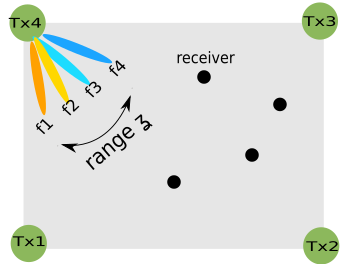
\includegraphics[width=0.3\textwidth]{environment.png}
\caption{Environment}
\label{fig:environment}
\end{figure}


\begin{small}
\begin{center}
\begin{tabular}{ c c }
\hline
Number of Energy Transmitting Nodes & L=4\\
\hline
&$TX_1$(0,0)\\
&$TX_2$(30,0)\\
{Positions of Trasmitting Node}&$TX_3$(30,30)\\
&$TX_4$(0,30)\\
\hline
Number of Radiation Elements per Trasmitting Node & M=64\\
\hline
Energy Carrier Frequency & 8M Hz\\
\hline
Field of Energy Receivers & 30m x 30m\\
\hline
Number of Energy Receivers & K \\
\hline
Energy Transfer Time & 0.5s \\
\hline
Information Transfer Time & 0.5s\\
\hline
Maximum Number of Steps & 100\\
\hline

\end{tabular}
\end{center}
\end{small}

Observation Space:\{$e_1,e_2,...e_K,c_1,c_2,c_3,c_4$\}
where $e_j$ is the energy received at the $j^{th}$ receiver, $c_i$ is the codebook choice for the $i^{th}$ energy emitting node.

Reward: If $e_j$ < $e_min$, reward is deducted by 50 points each. If $e_{total}^new$ > $e_{total}^new$, reward is increased by 100 points. If $e_{total}^new$ < $e_{total}^new$, reward is deduced by 300 points.

\subsection{A3C agent}
\begin{small}
\begin{center}
\begin{tabular}{ c c }
\hline
Layers of Actor Network & 3\\
\hline
Layers of Critic Network & 3\\
\hline
Learning Rate for Actor & $\alpha_a$=0.1\\
\hline
Learning Rate for Critic & $\alpha_c$=0.1\\
\hline
Discount Rate & $\gamma$=0.9 \\
\hline
Action Function & Softmax \\
\hline

\end{tabular}
\end{center}
\end{small}

\subsection{Simulation Result}
\section{Conclusion}
In this paper, we demonstrated the possibility to formulate WPT as a multiagent reinforcement learning problem, this lays the groundwork for further study towards fully locally computed control algorithms for wirelessly powered communication networks. Instead of group actions of all agents together, a multiagent rollout approach sees things sequentially, action taken by one agent becomes part of the state of another. This framework deduces the dimension of action space from exponential growth to multiplicative growth, and it can be applied to other problems. The most recent incarceration of beamforming technology is a passive reflective surface, or Intelligent Reflective Surface(IRS), where the reflective components are in the thousands. The multiagent approach proposed in this paper could be applied to IRS control as well, which should be a fruitful topic of future studies.






\bibliographystyle{IEEEtran}
\bibliography{Bibliography}
%\printbibliography



\end{document}
